\title{BT5110 Data Management and Warehousing}

\subtitle{Tutorial 1: Creating \& Populating Tables with Constraints}

\author{Mark Meng Huasong}

\institute[National University of Singapore] % (optional, but mostly needed)
{
	School of Computing\\
	National University of Singapore
}

\titlegraphic{
	
\includegraphics[width=2cm]{nus-logo}
}

\date{Aug 2021}

\begin{frame}
	\titlepage
\end{frame}

\section*{Greeting!}

\begin{frame}[fragile]{Greeting!}
Welcome to BT5110!\vspace{15pt}

\textbf{Mark MENG Huasong} (
\includegraphics[height=\fontcharht\font`\B]{t1/images/chn-chars.png}) \vspace{15pt}

B.Eng.(Hons), Computer Science, Nanyang Technological University

M.Comp., Infocomm Security, National University of Singapore\vspace{15pt}

Been in cyber-security R\&D industry since 2014, came back NUS for PhD in 2019\vspace{15pt}

I will be your TA for the first half of the semester!
\end{frame}

\section*{Question 1}

\begin{frame}[fragile]{Question 1 (a-c)}
(a) Download the following files from Luminus ``Files > Cases > Book Exchange''.
\begin{itemize}
	\item[] \texttt{NUNStASchema.sql},
	\item[] \texttt{NUNStAStudent.sql},
	\item[] \texttt{NUNStABook.sql},
	\item[] \texttt{NUNStACopy.sql},
	\item[] \texttt{NUNStALoan.sql}, and \texttt{NUNStAClean.sql}.
\end{itemize}
\vspace{10pt}

(b) Read the SQL files. What are they doing? \vspace{10pt}

(c) Use the files to create and populate a database (they may need some bug fixing).
\end{frame}

\begin{frame}[fragile]{Solution 1 (b)}
\begin{figure}
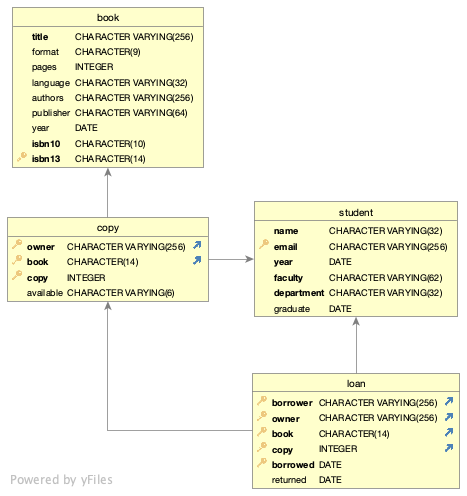
\includegraphics[width=0.6\textwidth]{t1/images/t1-0.png}
\caption{ER Diagram of NUNStASchema (plotted by DbVisualizer)}
\end{figure}
\end{frame}

\begin{frame}[fragile]{Solution 1 (b) Cont.}

\begin{columns}
\column{0.65\textwidth}
The first file to be run is \texttt{NUNStASchema.sql}. It creates the different tables. The referential integrity constraints (\texttt{FOREIGN KEY}) impose that the table \texttt{copy} and the table \texttt{loan} are created after the tables \texttt{student} and \texttt{book} and in that order.\vspace{10pt}

The table \texttt{student} is populated using \texttt{NUNStAStudent.sql}. \vspace{10pt}

The table \texttt{book} is populated using \texttt{NUNStABook.sql}. \vspace{10pt}

\textbf{\textit{These two tables can be populated in any order.}} 

\column{0.35\textwidth}
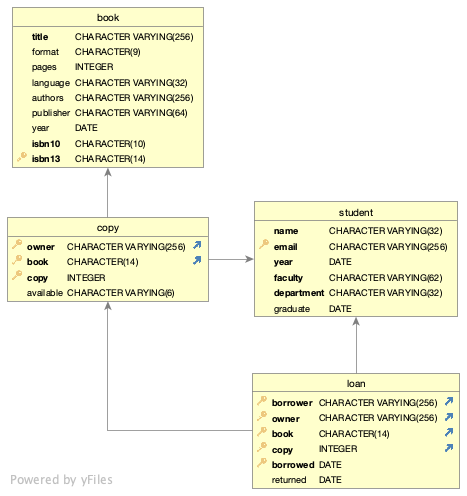
\includegraphics[width=\textwidth]{t1/images/t1-0.png}
\end{columns}
\end{frame}

\begin{frame}[fragile]{Solution 1 (b) Cont.}

\begin{columns}
\column{0.65\textwidth}
The table \texttt{copy} is populated using \texttt{NUNStACopy.sql}. \vspace{10pt}

The table \texttt{loan} is populated using \texttt{NUNStALoan.sql}. \vspace{10pt}

\textit{\textbf{The table \texttt{copy} and the table \texttt{loan} can only be populated after the tables \texttt{student} and \texttt{book} are populated and in that order because of the referential integrity constraints (\texttt{FOREIGN KEY}).} } \vspace{10pt}

The referential integrity constraints (\texttt{FOREIGN KEY}) impose that the table \texttt{loan} and the table \texttt{copy} are deleted before the tables \texttt{student} and \texttt{book} and in that order in \texttt{NUNStAClean.sql} matters.

\column{0.35\textwidth}
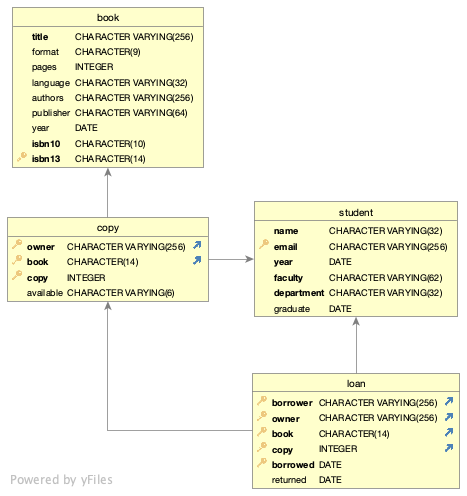
\includegraphics[width=\textwidth]{t1/images/t1-0.png}
\end{columns}

\end{frame}

\begin{frame}[fragile]{Solution 1 (c)}

There is a bug in \texttt{NUNStASchema.sql}, as the populating order of table \texttt{loan} (line 29-39) and \texttt{copy} (line 41-47) are wrong. \vspace{10pt}

You can fix it by \textbf{\textit{swapping}} these two code sections.\vspace{10pt}

Then execute all SQL files except \texttt{NUNStAClean.sql} through PgAdmin.

\begin{alertblock}{Notice}
You need to execute all those SQL files except \texttt{NUNStAClean.sql} for the sequential quesitons.
\end{alertblock}
\end{frame}

\section*{Question 2}

\begin{frame}[fragile]{Question \& Solution 2 (a)}
Insert the following new book.

\begin{lstlisting}
INSERT INTO book VALUES (
	'An Introduction to Database Systems',
	'paperback' , 
	640 , 
	'English' , 
	'C. J. Date' , 
	'Pearson',
	'2003-01-01' , 
	'0321197844' , 
	'978-0321197849');
\end{lstlisting} 


\textbf{Solution}: Notice the implicit order of the fields.

You can check that the insertion was effective with the following query.
\begin{lstlisting}
SELECT * FROM book;
\end{lstlisting}

\end{frame}

\begin{frame}[fragile]{Question \& Solution 2 (b)}
Insert the same book with a different \texttt{ISBN13}, for instance \texttt{'978-0201385908'}. \vspace{10pt}

\textbf{Solution}: Execute the code bellow:

\begin{lstlisting}
INSERT INTO book VALUES (
	'An Introduction to Database Systems', 
	'paperback', 
	640,
	'English',
	'C.J. Date', 
	'Pearson', 
	'2003-01-01', 
	'0321197844',  
	'978-0201385908');
\end{lstlisting}

\textcolor{brown}{Can you spot the problem in this code?}
\end{frame}

\begin{frame}[fragile]{Solution 2 (b) Cont.}

The command yields an error because \texttt{ISBN10} must be unique. PostgreSQL returns the following error message.

\begin{lstlisting}[style=error]
ERROR:  duplicate key value violates unique constraint "book_isbn10_key"
DETAIL:  Key (isbn10)=(0321197844) already exists.
SQL state: 23505
\end{lstlisting}

\begin{block}{Remark} 
All messages emitted by the PostgreSQL server are assigned five-character error codes that follow the SQL standard's conventions for ``SQLSTATE'' codes. Applications that need to know which error condition has occurred should usually test the error code, rather than looking at the textual error message. \vspace{10pt}

See \url{www.postgresql.org/docs/13/errcodes-appendix.html}
\end{block}
\end{frame}

\begin{frame}[fragile]{Question \& Solution 2 (c)}
Insert the same book  with the original \texttt{ISBN13} but with a different \texttt{ISBN10}, for instance \texttt{'0201385902'}.\vspace{10pt}

\textbf{Solution}: Execute the code bellow:

\begin{lstlisting}
INSERT INTO book VALUES (
	'An Introduction to Database Systems', 
	'hardcover',
	938,
	'English',
	'C.J. Date',
	'Addison Wesley Longman',
	'2000-01-01',
	'0201385902',
	'978-0321197849');
\end{lstlisting}

\textcolor{brown}{Will this code work?}
\end{frame}

\begin{frame}[fragile]{Solution 2 (c) Cont.}

The command yields an error  because  \texttt{ISBN13} is a primary key and therefore unique. PostgreSQL returns the following error message.

\begin{lstlisting}[style=error]
ERROR:  duplicate key value violates unique constraint "book_pkey"
DETAIL:  Key (isbn13)=(978-0321197849) already exists.
SQL state: 23505
\end{lstlisting}
\end{frame}

\begin{frame}[fragile]{Question \& Solution 2 (d)}
Insert the following new student.

\begin{lstlisting}
INSERT INTO student VALUES (
	'TIKKI TAVI' , 
	'tikki@gmail.com' , 
	'2010-01-01', 
	'School of Computing', 
	'CS', 
	NULL);
\end{lstlisting}

Notice that the value of the field \texttt{year} is \texttt{NULL}. This is because the student has not yet graduated.
\end{frame}

\begin{frame}[fragile]{Question \& Solution 2 (e)}
Insert the following new student.

\begin{lstlisting}
INSERT INTO student (email, name, year, faculty, department)
	VALUES (
	'rikki@gmail.com', 
	'RIKKI TAVI', 
	'2010-01-01',
	'School of Computing', 
	'CS');
\end{lstlisting}

Notice how we explicitly indicate the order of the fields in the insertion command. In this case, if a field is omitted, the system attempts to insert a null value.

\end{frame}

\begin{frame}[fragile]{Question \& Solution 2 (e) Cont.}
\textbf{Extra}: How about the following code (insertion).
\begin{lstlisting}
INSERT INTO student (name, year, faculty, department) 
	VALUES (
	'RIKKI TAVI',  
	'2010-01-01', 
	'School of Computing', 
	'CS');
\end{lstlisting}

\textcolor{brown}{Is this code okay?}
\end{frame}

\begin{frame}[fragile]{Question \& Solution 2 (e) Cont.}
The command does not work because \texttt{email} is a primary key and therefore cannot be null.

\begin{lstlisting}[style=error]
ERROR:  null value in column "email" violates not-null constraint
DETAIL:  Failing row contains (RIKKI TAVI, null, 2010-01-01, 
School of Computing, CS, null).
SQL state: 23502
\end{lstlisting}
\end{frame}


\begin{frame}[fragile]{Question \& Solution 2 (f)}
Change the name of the department 'CS' to 'Computer Science'.

\begin{lstlisting}
UPDATE student
SET department = 'Computer Science'
WHERE department = 'CS';
\end{lstlisting}

You can check that the update was effective with the following queries.
The first query has no result.
\begin{lstlisting}
SELECT * FROM student WHERE department = 'CS';
\end{lstlisting}

The second query prints the students from the computer science department.
\begin{lstlisting}
SELECT * FROM student WHERE department = 'Computer Science';
\end{lstlisting}
\end{frame}

\begin{frame}[fragile]{Question \& Solution 2 (g)}
Delete the students from the 'chemistry' department.

\begin{lstlisting} 
DELETE FROM student 
WHERE department = 'chemistry';
\end{lstlisting}

`chemistry' is misspelled with a lower case `c'. There is no error but nothing is deleted because there is no department `chemistry'.
\end{frame}

\begin{frame}[fragile]{Question \& Solution 2 (h)}
Delete the students from the 'Chemistry' department.

\begin{lstlisting}
DELETE FROM student 
WHERE department = 'Chemistry';
\end{lstlisting}

\textcolor{brown}{Will this code work?}
\end{frame}

\begin{frame}[fragile]{Question \& Solution 2 (h) Cont.}

Nothing is deleted because a constraint is \textbf{violated}. It is not a programming error. It is part of the control of the access to the data.
\begin{lstlisting}[style=error]
ERROR:  update or delete on table "student" violates foreign key constraint "loan_borrower_fkey" on table "loan"
DETAIL:  Key (email)=(xiexin2011@gmail.com) is still referenced from table "loan".
SQL state: 23503
\end{lstlisting}
\end{frame}


\section*{Question 3}

\begin{frame}[fragile]{Question \& Solution 3 (a)}
Some constraints in PostgreSQL are \texttt{DEFERRABLE}. What does it mean? \vspace{10pt}

Upon creation, a \texttt{UNIQUE}, \texttt{PRIMARY KEY}, or \texttt{FOREIGN KEY} constraint is given one of three characteristics: \texttt{DEFERRABLE} \texttt{INITIALLY IMMEDIATE}, \texttt{DEFERRABLE INITIALLY DEFERRED}, and \texttt{NOT DEFERRABLE}.  \vspace{10pt}

By default the above constraints and all others are \textcolor{red}{\texttt{NOT DEFERRABLE}}. A \texttt{NOT DEFERRABLE} constraint is always \texttt{IMMEDIATE}. By default a \texttt{DEFERRABLE} constraint is \texttt{INITIALLY IMMEDIATE}. \vspace{10pt}

These qualifications refers to when the constraint is checked: immediately after each operation (\texttt{INSERT}, \texttt{DELETE}, \texttt{UPDATE}), or at the end of the transaction executing the operation. \vspace{10pt}

Although this is not the default setting, it is preferable that all constraints be \textcolor{red}{deferred}. Unfortunately, this is only possible for \texttt{UNIQUE}, \texttt{PRIMARY KEY}, and \texttt{FOREIGN KEY} constraints and not for \texttt{CHECK} constraints in the current version of PostgreSQL.
\end{frame}


\begin{frame}[fragile]{Question \& Solution 3 (b)}
Insert the following copy of 'An Introduction to Database Systems' owned by Tikki. \vspace{10pt}

\begin{lstlisting}
INSERT INTO copy VALUES (
	'tikki@gmail.com', 
	'978-0321197849', 
	1, 
	'TRUE') ;
\end{lstlisting}

What is the difference between the following two SQL programs?
\end{frame}


\begin{frame}[fragile]{Question \& Solution 3 (b) Cont.}
	\begin{lstlisting}
		BEGIN TRANSACTION;
		SET CONSTRAINTS ALL IMMEDIATE;
		DELETE FROM book WHERE ISBN13 = '978-0321197849' ;
		DELETE FROM copy WHERE book = '978-0321197849' ;
		END TRANSACTION;
	\end{lstlisting}
	
	\begin{lstlisting}
		BEGIN TRANSACTION;
		SET CONSTRAINTS ALL DEFERRED;
		DELETE FROM book WHERE ISBN13 = '978-0321197849' ;
		DELETE FROM copy WHERE book = '978-0321197849' ;
		END TRANSACTION;
	\end{lstlisting}
\textcolor{brown}{What is the difference between these two SQL programs?}
\end{frame}


\begin{frame}[fragile]{Question \& Solution 3 (b) Cont.}
\begin{lstlisting}
BEGIN TRANSACTION;
SET CONSTRAINTS ALL IMMEDIATE;
DELETE FROM book 
WHERE ISBN13 = '978-0321197849' ;
DELETE FROM copy 
WHERE book = '978-0321197849' ;
END TRANSACTION;
\end{lstlisting}

In the first transaction, the statement \texttt{SET CONSTRAINTS ALL IMMEDIATE;} checks the reference from the table \texttt{copy} to the table \texttt{book} checkable after each operation. The first deletion of the transaction violates the constraint.

\begin{lstlisting}[style=error]
ERROR:  current transaction is aborted, commands ignored until end of transaction block
SQL state: 25P02
\end{lstlisting}

\end{frame}


\begin{frame}[fragile]{Question \& Solution 3 (b) Cont.}
This is the default, so the code below has the same issue.

\begin{lstlisting}
BEGIN TRANSACTION;
DELETE FROM book 
WHERE ISBN13 = '978-0321197849';
DELETE FROM copy 
WHERE book = '978-0321197849';
END TRANSACTION;
\end{lstlisting}

When the execution is interrupted, you need to run ``\texttt{END TRANSACTION;}'' {\color{red} \textbf{\textit{manually}}}. \vspace{10pt}

You can also use commands like \texttt{BEGIN}, \texttt{COMMIT} as well as  \texttt{SAVEPOINT my\_savepoint} and \texttt{ROLLBACK TO my\_savepoint;} to control the flow of transactions.

\end{frame}


\begin{frame}[fragile]{Question \& Solution 3 (b) Cont.}

\begin{lstlisting}
BEGIN TRANSACTION;
SET CONSTRAINTS ALL DEFERRED;
DELETE FROM book WHERE ISBN13 = '978-0321197849' ;
DELETE FROM copy WHERE book = '978-0321197849' ;
END TRANSACTION;
\end{lstlisting}

In the second transaction, the constraints are checked at the end of the transaction and are not violated.  Namely, \texttt{SET CONSTRAINTS ALL DEFERRED} makes the reference from the table \texttt{copy} to the table \texttt{book} checkable at the end of transactions. The combined effect of the two deletions in the transaction does not violate the FOREIGN KEY constraint. The transaction is committed. \vspace{10pt}

Note that SQLite has a pragma called \texttt{defer\_foreign\_keys} to control deferred foreign keys.
\end{frame}

\section*{Question 4}

\begin{frame}[fragile]{Question \& Solution 4 (a)}
Argue that there is no need for the \texttt{available} field of the table \texttt{copy}. Make the necessary changes.
\begin{columns}
	\column{0.45\textwidth}
\textcolor{brown}{Do you agree with that? Why?}\\
\textcolor{brown}{Any potential issue if we keep it?}
\column{0.5\textwidth}
\begin{figure}
	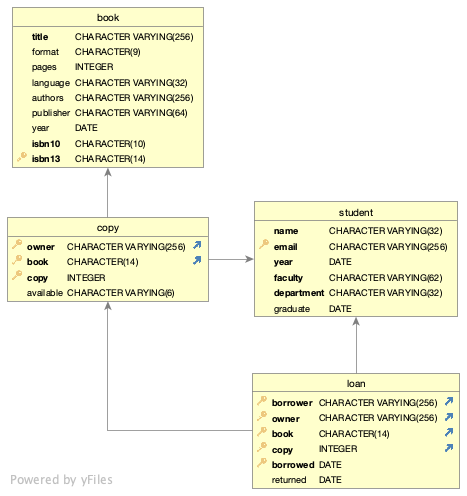
\includegraphics[width=1\textwidth]{t1/images/t1-0.png}
\end{figure}
\end{columns}

\end{frame}

\begin{frame}[fragile]{Question \& Solution 4 (a) Cont.}
\textbf{Solution}:
The availability of a copy can be derived. \vspace{10pt}
The following query finds the copies loaned but not returned and therefore not available.
\begin{lstlisting}
SELECT owner, book, copy, returned 
FROM loan 
WHERE returned ISNULL;
\end{lstlisting}

We drop the \texttt{available} field in the table \texttt{copy}

\begin{lstlisting}
ALTER TABLE copy
DROP COLUMN available;
\end{lstlisting}

\end{frame}

\begin{frame}[fragile]{Question \& Solution 4 (a) Cont.}
\textbf{Extra}: We could even create a view \texttt{copy\_view} with the field restored.

\begin{lstlisting}
CREATE OR REPLACE VIEW copy_view (owner, book, copy, available) 
AS (SELECT DISTINCT c.owner, c.book, c.copy, 
CASE
	WHEN EXISTS (SELECT * FROM loan l  
	WHERE l.owner = c.owner
		AND l.book = c.book
		AND l.copy = c.copy 
		AND l.returned ISNULL) 
	THEN 'FALSE'
	ELSE 'TRUE' 
END
FROM copy c);

SELECT * FROM copy_view;
\end{lstlisting}

\end{frame}

\begin{frame}[fragile]{Question \& Solution 4 (a) Cont.}
Can the view be updated? 

\begin{lstlisting}
UPDATE copy_view 
SET owner = 'tikki@google.com' 
WHERE owner = 'tikki@gmail.com'
\end{lstlisting}

In principle we should be able to update all fields except \texttt{available}.  \vspace{10pt}

It is however not directly possible but it can be programmed using \texttt{INSTEAD OF UPDATE} triggers or  unconditional \texttt{ON UPDATE DO INSTEAD} rules.

\begin{lstlisting}
DROP VIEW copy_view;
\end{lstlisting}
\end{frame}

\begin{frame}[fragile]{Question \& Solution 4 (b)}
Argue that the table \texttt{student} should not contain both the fields \texttt{department} and \texttt{faculty}. Make the necessary changes. \vspace{10pt}

\textcolor{brown}{Do you agree with that? Why?}\\
\end{frame}

\begin{frame}[fragile]{Question \& Solution 4 (b) Cont.}

\textbf{Solution}:
The faculty is determined by the department. This information can be stored once and for all in a separate table. The student table needs only to store the department. \vspace{10pt}

The changes can be done with the following SQL code.

\begin{lstlisting}
CREATE TABLE department (
	department VARCHAR(32) PRIMARY KEY,
	faculty VARCHAR(62) NOT NULL);

INSERT INTO department 
SELECT DISTINCT department, faculty FROM student;

ALTER TABLE student DROP COLUMN faculty;

ALTER TABLE student
ADD FOREIGN KEY (department) REFERENCES department(department);
\end{lstlisting}
\end{frame}


\begin{frame}[fragile]{End of Tutorial 1}
	Below is what your database (should) be like by the end of this tutorial:
	
	\begin{figure}
		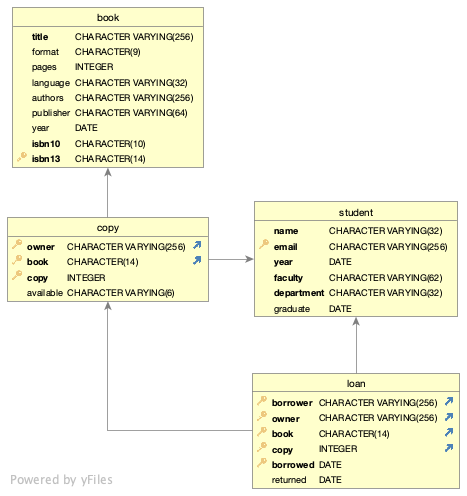
\includegraphics[width=0.6\textwidth]{t1/images/t1-0.png}
	\end{figure}
 (plotted by DbVisualizer)
\end{frame}

\section*{Project 1}

\begin{frame}[fragile]{Submission due this week}
	(a) Your project 1 (Generating fake but realistic data) is due on this Friday 5:00PM (SGT)
	\\ \textcolor{red}{\scriptsize(not Anytime on Earth, not 11:59PM, not sure the LumiNus and Internet work well at the last minute)}.\vspace{10pt}
	
	(b) Double check your code! Never lose any mark due to \textbf{typo} and \textbf{missing semicolons} (;) \vspace{10pt}
	
	(c) Creativity and ``code cleanness'' are always appreciated.
	\\ \textcolor{red}{\scriptsize(extremely important since you are business students :D)}.\vspace{10pt}
\end{frame}
\section*{Project 1}

\begin{frame}[fragile]{Submission due this week: Code Cleanness}
	Just an example! There are lots of free tools online for you to take advantage... \vspace{10pt}
	\begin{figure}
		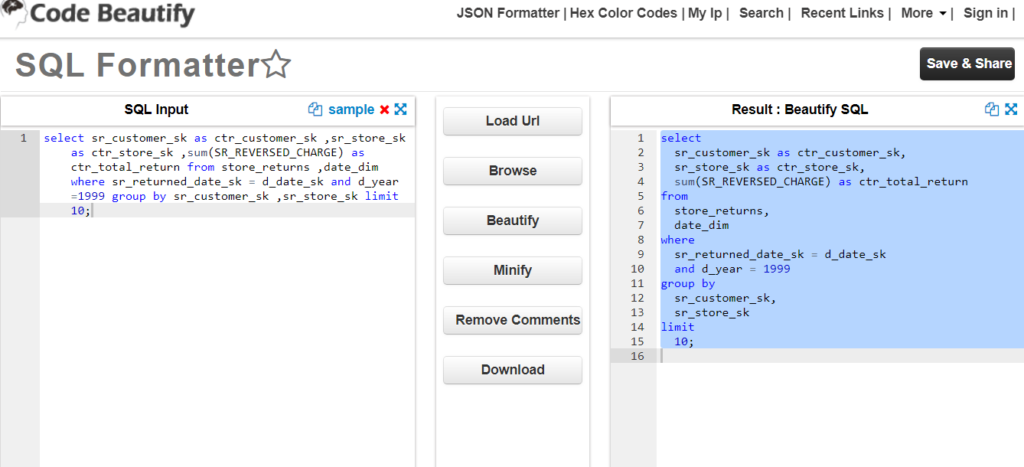
\includegraphics[width=0.75\textwidth]{t1/images/code_format.png}
	\end{figure}
\end{frame}

\begin{frame}{}
\centering  
For any further question, please feel free to email me:\vspace{10pt}

huasong.meng@u.nus.edu \vspace{20pt}

See you next week!
\end{frame}